% ======================================================================
%  3. Separation of concerns: target matching
% ======================================================================
\section{Separation of concerns: target matching}
\label{sec:contrib-tm}

Target matching is the smallest non-trivial instance of the separation-of-concerns
question, and the one where the modelling boundary can be analysed most sharply.
The goal is not to maximize $f$ but to reach a prescribed level: given a scalar
target $T$, solve
\begin{equation}
  \min_{x\in\X}\; g(x), \qquad g(x):=\abs{f(x)-T}.
  \label{eq:tm-problem}
\end{equation}
In the laboratory this is the natural formalization of ``find a stimulation that
produces a prescribed neural response''.

\subsection{Two formulations}
\label{sec:contrib-tm-two}

The two architectures of Section~\ref{sec:intro-soc} instantiate as follows.

\paragraph{Separated / \RIGHT.}
The GP models the \emph{raw} phenomenon $f$ (trained on the raw observations
$y_t$); the target enters only the acquisition. Pushing the confidence interval
on $f$ through the distance-to-target map gives
\begin{equation}
  a_t^{\RIGHT}(x) \;=\; -\inf_{z\in C_t(x)}\abs{z-T},
  \label{eq:tm-right-full}
\end{equation}
where $C_t(x)=[\mu_{t-1}(x)-\sqrt{\beta_t}\sigma_{t-1}(x),\,
\mu_{t-1}(x)+\sqrt{\beta_t}\sigma_{t-1}(x)]$ is the GP confidence interval. A
convenient closed form used in the experiments is
\begin{equation}
  a_t^{\mathrm{TM}}(x) \;=\; -\abs{\mu_{t-1}(x)-T}+\sqrt{\beta_t}\,\sigma_{t-1}(x),
  \label{eq:tm-right-simple}
\end{equation}
which is attractive where the posterior mean is close to $T$, with an exploration
bonus for high uncertainty.

\paragraph{Task-in-model / \WRONG.}
The GP is trained on the \emph{transformed} observations $\abs{y_t-T}$, so it
models $\abs{f-T}$ directly, and the acquisition is a lower confidence bound on
this surrogate. The target is baked into the training data --- and, as we now
show, into the regularity the surrogate is asked to have.

\subsection{From a qualitative obstruction to a quantitative barrier}
\label{sec:contrib-tm-barrier}

The theoretical development proceeds in four steps. It is the step from
\emph{qualitative} to \emph{quantitative} that we regard as the main contribution.

\paragraph{Step 1 --- a transverse crossing creates a cusp.}
Assume a transverse target crossing at $x_0$: $f(x_0)=T$ and $\nabla f(x_0)\neq0$.
Locally $\abs{f(x)-T}\approx\abs{\nabla f(x_0)^\top(x-x_0)}$, which has a cusp
along the level set $\{f=T\}$ (Figure~\ref{fig:tm-cusp}). The absolute value
folds a smooth transverse crossing into a non-differentiable ridge exactly where
the optimum lies.

\paragraph{Step 2 --- qualitative non-membership.}
Combining the cusp with a smooth-kernel assumption gives a first, qualitative
obstruction.

\begin{proposition}[Loss of regularity, {proof in Appendix~\ref{app:tm}}]
\label{prop:tm-nonmember}
Let $k$ be a kernel with $\Hk\subset C^1(\X)$, and let $g=\abs{f-T}$ with
$f\in C^1(\X)$. If there exists $x_0$ with $f(x_0)=T$ and $\nabla f(x_0)\neq0$,
then $g$ is not differentiable at $x_0$; in particular $g\notin\Hk$.
\provbadge{colContrib}{personal contribution}
\end{proposition}

The transversality condition $\nabla f(x_0)\neq0$ is essential: if
$\nabla f(x_0)=0$ the level set may be tangent and $\abs{f-T}$ can remain smooth
(e.g.\ $f(x)=x^2$, $T=0$). A general normal-form analysis
(Appendix~\ref{app:tm}) shows the singularity created by a transverse kink sits
exactly at the Sobolev threshold $s=3/2$, and locates the corresponding
non-membership for Mat\'ern kernels via $\nu+d/2\ge q+\tfrac12$.

\paragraph{Step 3 --- why non-membership is too weak.}
As emphasized in Section~\ref{sec:bg-misspec}, $g\notin\Hk$ does not imply that
the algorithm cannot converge: an out-of-RKHS function can still be uniformly
approximated to arbitrary accuracy by RKHS functions (by mollification), and the
$\eps$-misspecified theory of Bogunovic--Krause~\cite{bogunovic2021} degrades
only in the achievable approximation level. The right question is therefore
quantitative: \emph{at what price, in RKHS norm, can $g$ be approximated?}

\paragraph{Step 4 --- the quantitative approximation problem.}
This leads to the central quantity
\begin{equation}
  \epsinf(B) \;:=\; \inf_{\Hnorm{h}\le B}\;\norm{h-g}_\infty,
  \label{eq:tm-epsinf}
\end{equation}
the best sup-norm approximation of the task-transformed objective by an RKHS ball
of radius $B$. The main theoretical result of this section lower-bounds
$\epsinf(B)$: complexity must grow to buy accuracy, and it must grow fast.

\begin{theorem}[Approximation barrier, {proof in Appendix~\ref{app:tm}}]
\label{thm:tm-barrier}
Let $g=\abs{f-T}$ with $f\in C^2$, $f(x_0)=T$, $\nabla f(x_0)\neq0$, and let $k$
be a $\tau_k$-regular kernel with $\nu:=\tau_k-\tfrac d2>1$, so that the Sobolev
embedding gives $\Hk\hookrightarrow C^\nu$ with
$\norm{h}_{C^\nu}\le C_S\Hnorm{h}$. Then there exist $c>0$ and $B_0$ such that
for all $B\ge B_0$,
\begin{equation}
  \epsinf(B)\;\ge\; c\,B^{-1/(\nu-1)}.
  \label{eq:tm-barrier}
\end{equation}
In dimension $d=1$, mollification provides a matching upper bound, so
$\epsinf(B)\asymp B^{-1/(\nu-1)}$.
\provbadge{colContrib}{personal contribution}
\end{theorem}

\begin{remark}[Geometric intuition]
The obstruction is local, and it lives exactly where accuracy matters --- at the
optimizer, on the level set. A finite even-order finite difference of $\abs{u}$
at the kink is bounded below by a positive multiple of the step, while for an
RKHS function of $C^\nu$ regularity the same finite difference is
$O(\text{step}^\nu)$; balancing the two in the step size, and using
$\norm{h}_{C^\nu}\lesssim B$, yields~\eqref{eq:tm-barrier}. The rate collapses as
$\nu\downarrow1$: a rougher kernel finds the kink easier to represent, which is
consistent with viewing the phenomenon through a kernel matched to its true
regularity. The full finite-difference / mollification proof is deferred to
Appendix~\ref{app:tm}. The RBF kernel is excluded from the polynomial statement
because its RKHS is not a finite-order Sobolev space; qualitatively, an analytic
kernel is even more strongly penalized by a cusp.
\end{remark}

\begin{remark}[Beyond absolute target matching]
The mechanism behind Theorem~\ref{thm:tm-barrier} is not specific to the absolute-value transformation. What matters is the creation of a first-order kink. More generally, let $g=\rho\circ f$ and assume that, for some $x_0$ and some direction $v$, the one-sided directional derivatives of $g$ satisfy $D_v^+ g(x_0)-D_v^- g(x_0)\neq 0.$ Then the same finite-difference argument applies: the kink produces a contribution of order $s$, whereas any $h\in\Hk\hookrightarrow C^\nu$ with $\Hnorm{h}\le B$ has the corresponding finite difference bounded by $O(Bs^\nu)$. Balancing these terms again yields the scaling $\inf_{\Hnorm{h}\le B}\norm{h-g}_\infty
\gtrsim B^{-1/(\nu-1)}.$ Thus the approximation barrier should be understood as a consequence of a regularity mismatch induced by a non-smooth task transformation, rather than as a peculiarity of target matching. In particular, piecewise-$C^1$ transformations with a non-zero jump in slope across a task boundary fall under the same mechanism, provided the underlying phenomenon crosses that boundary transversally. Theorem~\ref{thm:tm-barrier} treats the target-matching case explicitly; the general formulation is left as a direct extension of the same argument.
\end{remark}


\begin{remark}[What the barrier is \emph{not}]
Theorem~\ref{thm:tm-barrier} is a statement about \emph{approximation}, not about
regret. Combined with a robust-misspecification upper bound such as
\cite{bogunovic2021} it says that the \emph{best available upper certificate} for
the task-in-model surrogate degrades; it does \emph{not} establish that
task-in-model GP-UCB incurs higher \emph{realized} regret than the separated
method, and it is not a lower regret bound. Constructing such a lower bound
remains open (Section~\ref{sec:discussion}).
\provbadge{colOpen}{open question}
\end{remark}

\begin{remark}{Complexity, lenghtscale, misspecification etc...}
    
\end{remark}

\figauto[0.62\linewidth]{figures/Theory/Barriere d'approximation.png}{%
  \textbf{Approximation barrier} $\epsinf(B)\gtrsim B^{-1/(\nu-1)}$ (log--log),
  one curve per smoothness $\nu$. The barrier collapses as $\nu\downarrow1$:
  rougher RKHSs represent the kink more cheaply. Illustrates
  Theorem~\ref{thm:tm-barrier}.}{fig:tm-barrier-plot}

\subsection{The positive result: separation preserves the GP-UCB guarantee}
\label{sec:contrib-tm-pos}

The separated formulation, by contrast, keeps the model well specified whenever
$f\in\Hk$ and pushes the intact confidence interval through the target-matching
map. This is enough to recover a GP-UCB-type guarantee.

\begin{theorem}[Separation of concerns for target matching, {proof in Appendix~\ref{app:tm}}]
\label{thm:tm-soc}
Let $k$ be a kernel with $f\in\Hk$, $\Hnorm{f}\le B$, observations
$y_t=f(x_t)+\eps_t$ with conditionally $R$-sub-Gaussian noise, and $\beta_t$
chosen so that the uniform confidence bound
$\abs{f(x)-\mu_{t-1}(x)}\le\sqrt{\beta_t}\sigma_{t-1}(x)$ holds with probability
$\ge 1-\delta$. Select $x_t\in\argmin_x a_t^{\mathrm{TM}}(x)$ with $a_t^{\mathrm{TM}}$
as in~\eqref{eq:tm-right-simple}. Then, with probability $\ge 1-\delta$, the
cumulative target-matching regret
$R_T^{\mathrm{TM}}=\sum_{t=1}^T\bigl(\abs{f(x_t)-T}-\abs{f(x^\star)-T}\bigr)$
satisfies
\begin{equation}
  R_T^{\mathrm{TM}} \;=\; O\!\left(\sqrt{T\,\beta_T\,\gain_T}\right).
  \label{eq:tm-soc}
\end{equation}
\provbadge{colContrib}{personal contribution}
\end{theorem}

The proof is a triangle-inequality pushforward: because $z\mapsto\abs{z-T}$ is
$1$-Lipschitz, the confidence interval on $f$ transports to a confidence interval
on the decision quantity, and the standard optimism argument then yields the same
per-step bound $r_t\le 2\sqrt{\beta_t}\sigma_{t-1}(x_t)$ as classical GP-UCB. The
task never touches the model; it is handled entirely in the decision. This is the
one-dimensional case of the general pushforward-confidence theorem we state for
multi-objective scalarizations in Section~\ref{sec:contrib-mo}.

\begin{takeaway}
$f$ may be smooth while $\abs{f-T}$ is not. Modelling $f$ and applying the target
in the acquisition keeps the model well specified and preserves the GP-UCB regret
rate; modelling $\abs{f-T}$ directly forces the surrogate to represent a cusp,
at a quantifiable RKHS cost.
\end{takeaway}



% ======================================================================
\subsection{Experiment A --- target matching}
\label{sec:contrib-tm-exp}

We now test the contrast empirically. \hfill\Pexp

\paragraph{Question / hypothesis.}
For a target-matching goal, does modelling the raw $f$ and applying the target in
the acquisition (\RIGHT) outperform modelling $\abs{f-T}$ directly (\WRONG),
and is the gap driven by the geometry of the transformed objective and by kernel
regularity?

\paragraph{Compared methods.}
Both are analytic, sequential ($q=1$) UCB-type acquisitions that multiply the
posterior standard deviation by $\sqrt{\beta_t}$. \RIGHT{}
(\texttt{right\_target\_matching\_ucb}) trains the GP on raw $y$ and maximizes
$-\abs{\mu-T}+\sqrt{\beta}\,\sigma$; \WRONG{} (\texttt{wrong\_gp\_on\_abs\_lcb})
trains on $\abs{y-T}$ and maximizes a lower confidence bound
$-\mu_g+\sqrt{\beta}\,\sigma_g$ on the transformed surrogate.

\paragraph{Benchmarks, dimension, target.}
Eight noiseless benchmarks span $d\in\{1,2,6\}$: monotone sanity checks
(\texttt{linear\_1d}, \texttt{exponential\_1d}); a family of deceptive
one-dimensional ``Gaussian trap'' functions (and thin/shifted/deep variants) that
keep $f$ regular while making the transformed geometry hard;
\texttt{branin\_2d} on the custom box $[0,5.5]\times[-2,6]$ with $T=5.0$; and
\texttt{hartmann\_6d} on $[0,1]^6$ with $T=-2.5$. Targets are attainable, so the
target-matching simple regret equals the best target distance found. A summary
table is given in Appendix~\ref{app:exp}.

\paragraph{Kernel and hyperparameter fitting.}
Mat\'ern-$5/2$ with ARD (BoTorch default, Gamma hyperpriors). Length-scale,
output-scale and constant mean are fit by exact marginal likelihood and
\emph{refit from scratch at every iteration}. Mat\'ern-$1/2$ and RBF are used
only in kernel-regularity ablations, to disentangle a specification bias from a
model/decision confusion.

\paragraph{Exploration schedule $\beta_t$.}
The theoretical, dimension-dependent \texttt{matern\_gamma} GP-UCB schedule
$\sqrt{\beta_t}=B+R\sqrt{2(\gain_{t-1}+1+\ln(1/\delta))}$ with
$B=1,R=1,\delta=0.1,\nu=2.5$, information-gain proxy scale $0.1$, applied
identically to \RIGHT{} and \WRONG. Some less conservative schedules of log beta and constant beta were also tested giving similar results.

\paragraph{Noise, input/output transforms.}
Noiseless observations ($\sigma=0$; a fixed-noise GP with variance floored to
$10^{-6}$). GP inputs are mapped to the unit cube; outputs are standardized and
re-fitted each iteration.

\paragraph{Initial design and budget.}
Scrambled Sobol initial design: $1$ point (1-D), $4$ (Branin), $12$ (Hartmann).
Budget $50$ evaluations ($100$ for Hartmann).

\paragraph{Seeds and acquisition optimization.}
$100$ independent seeds ($1$--$100$). Within a seed the Sobol design is drawn once
and the \emph{same} initial data is passed to both methods, which validates a
paired test. The seed fixes the Sobol scramble and the global torch RNG driving
the multi-start acquisition optimizer.

\paragraph{Metrics.}
Primary: target-matching simple regret
$\min_{t\le N}\abs{f(x_t)-T}-\min_x\abs{f(x)-T}$ on the noiseless $f$. Secondary:
running-best and instantaneous target distance, cumulative target regret, hitting
time and failure rate (final best distance above a threshold), plus probabilistic
calibration diagnostics (NLPD, empirical and near-target coverage, PIT,
confidence-violation rate) at snapshot checkpoints.

\paragraph{Aggregation and confidence.}
Median convergence curves with $95\%$ pointwise bootstrap bands ($10\,000$
resamples over seeds); primary comparison by paired one-sided Wilcoxon
signed-rank test (\RIGHT{} vs \WRONG), with Mann--Whitney~$U$, rank-biserial
correlation and Cohen's~$d$ as secondary effect sizes.

\paragraph{Results and interpretation.}
Three findings recur (Figures~\ref{fig:tm-cusp}--\ref{fig:tm-dims}).
\emph{(i) A controlled failure mode.} On the Gaussian trap, \WRONG{}'s posterior
keeps large uncertainty and a multi-modal acquisition and is repeatedly trapped
in a local basin of $\abs{f-T}$, whereas \RIGHT{} converges to the target by
$t\approx5$ (Figure~\ref{fig:trajectories}). \emph{(ii) Optimization is not the
whole story.} Beyond slower optimization, \WRONG{}'s posterior uncertainty
becomes unreliable near the target (degraded near-target coverage), so the issue
is also one of calibration, not only speed. \emph{(iii) Severity scales with
geometry and dimension.} On the trap the cumulative-regret gap is stark
(\WRONG{} grows roughly linearly while \RIGHT{} plateaus) and the failure rate at
threshold $0.015$ is $0.05$ (\RIGHT) versus $0.87$ (\WRONG); the gap persists but
narrows on Branin (2-D) and narrows further on Hartmann (6-D), where the
best-so-far panel becomes less conclusive. This is consistent with the barrier being
a \emph{local} obstruction whose practical bite depends on how often the
optimizer must resolve the cusp within the budget. \emph{(iv) The learned
surrogate becomes increasingly local.} In the misspecified model, the learned
lengthscale tends to decrease as the GP attempts to accommodate the sharp task
geometry, producing the characteristic saw-tooth posterior variance and
multi-modal acquisition between nearby observations. Although this is not
literally the growth of the fixed-kernel RKHS radius $B$ appearing in
Theorem~\ref{thm:tm-barrier}, it is consistent with the same underlying
complexity pressure: fitting the cusp requires an increasingly expressive
surrogate, here achieved by adapting the kernel itself rather than only by
increasing the norm budget within a fixed RKHS.


% --- Experiment A figures ----------------------------------------------


% --- Figures: the target-matching setup --------------------------------
\begin{figure}[htbp]
  \centering
  \begin{subfigure}[b]{0.48\linewidth}
    \centering\figph[\linewidth]{figures/EXPA/gaussian_trap.png}
    \caption{Raw $f$ with target line $T=0.38$ (modelled by \RIGHT).}
    \label{fig:tm-raw}
  \end{subfigure}\hfill
  \begin{subfigure}[b]{0.48\linewidth}
    \centering\figph[\linewidth]{figures/EXPA/gaussian_trap_abs.png}
    \caption{Transformed $\abs{f-T}$ with a kink at $x\approx0.62$ (modelled by \WRONG).}
    \label{fig:tm-abs}
  \end{subfigure}
  \caption{\textbf{The task transformation creates a cusp where the optimum lies.}
  A smooth phenomenon (left) becomes non-differentiable once folded through the
  distance-to-target map (right). This is the geometry behind
  Proposition~\ref{prop:tm-nonmember} and Theorem~\ref{thm:tm-barrier}.}
  \label{fig:tm-cusp}
\end{figure}

\begin{figure}
    \centering
    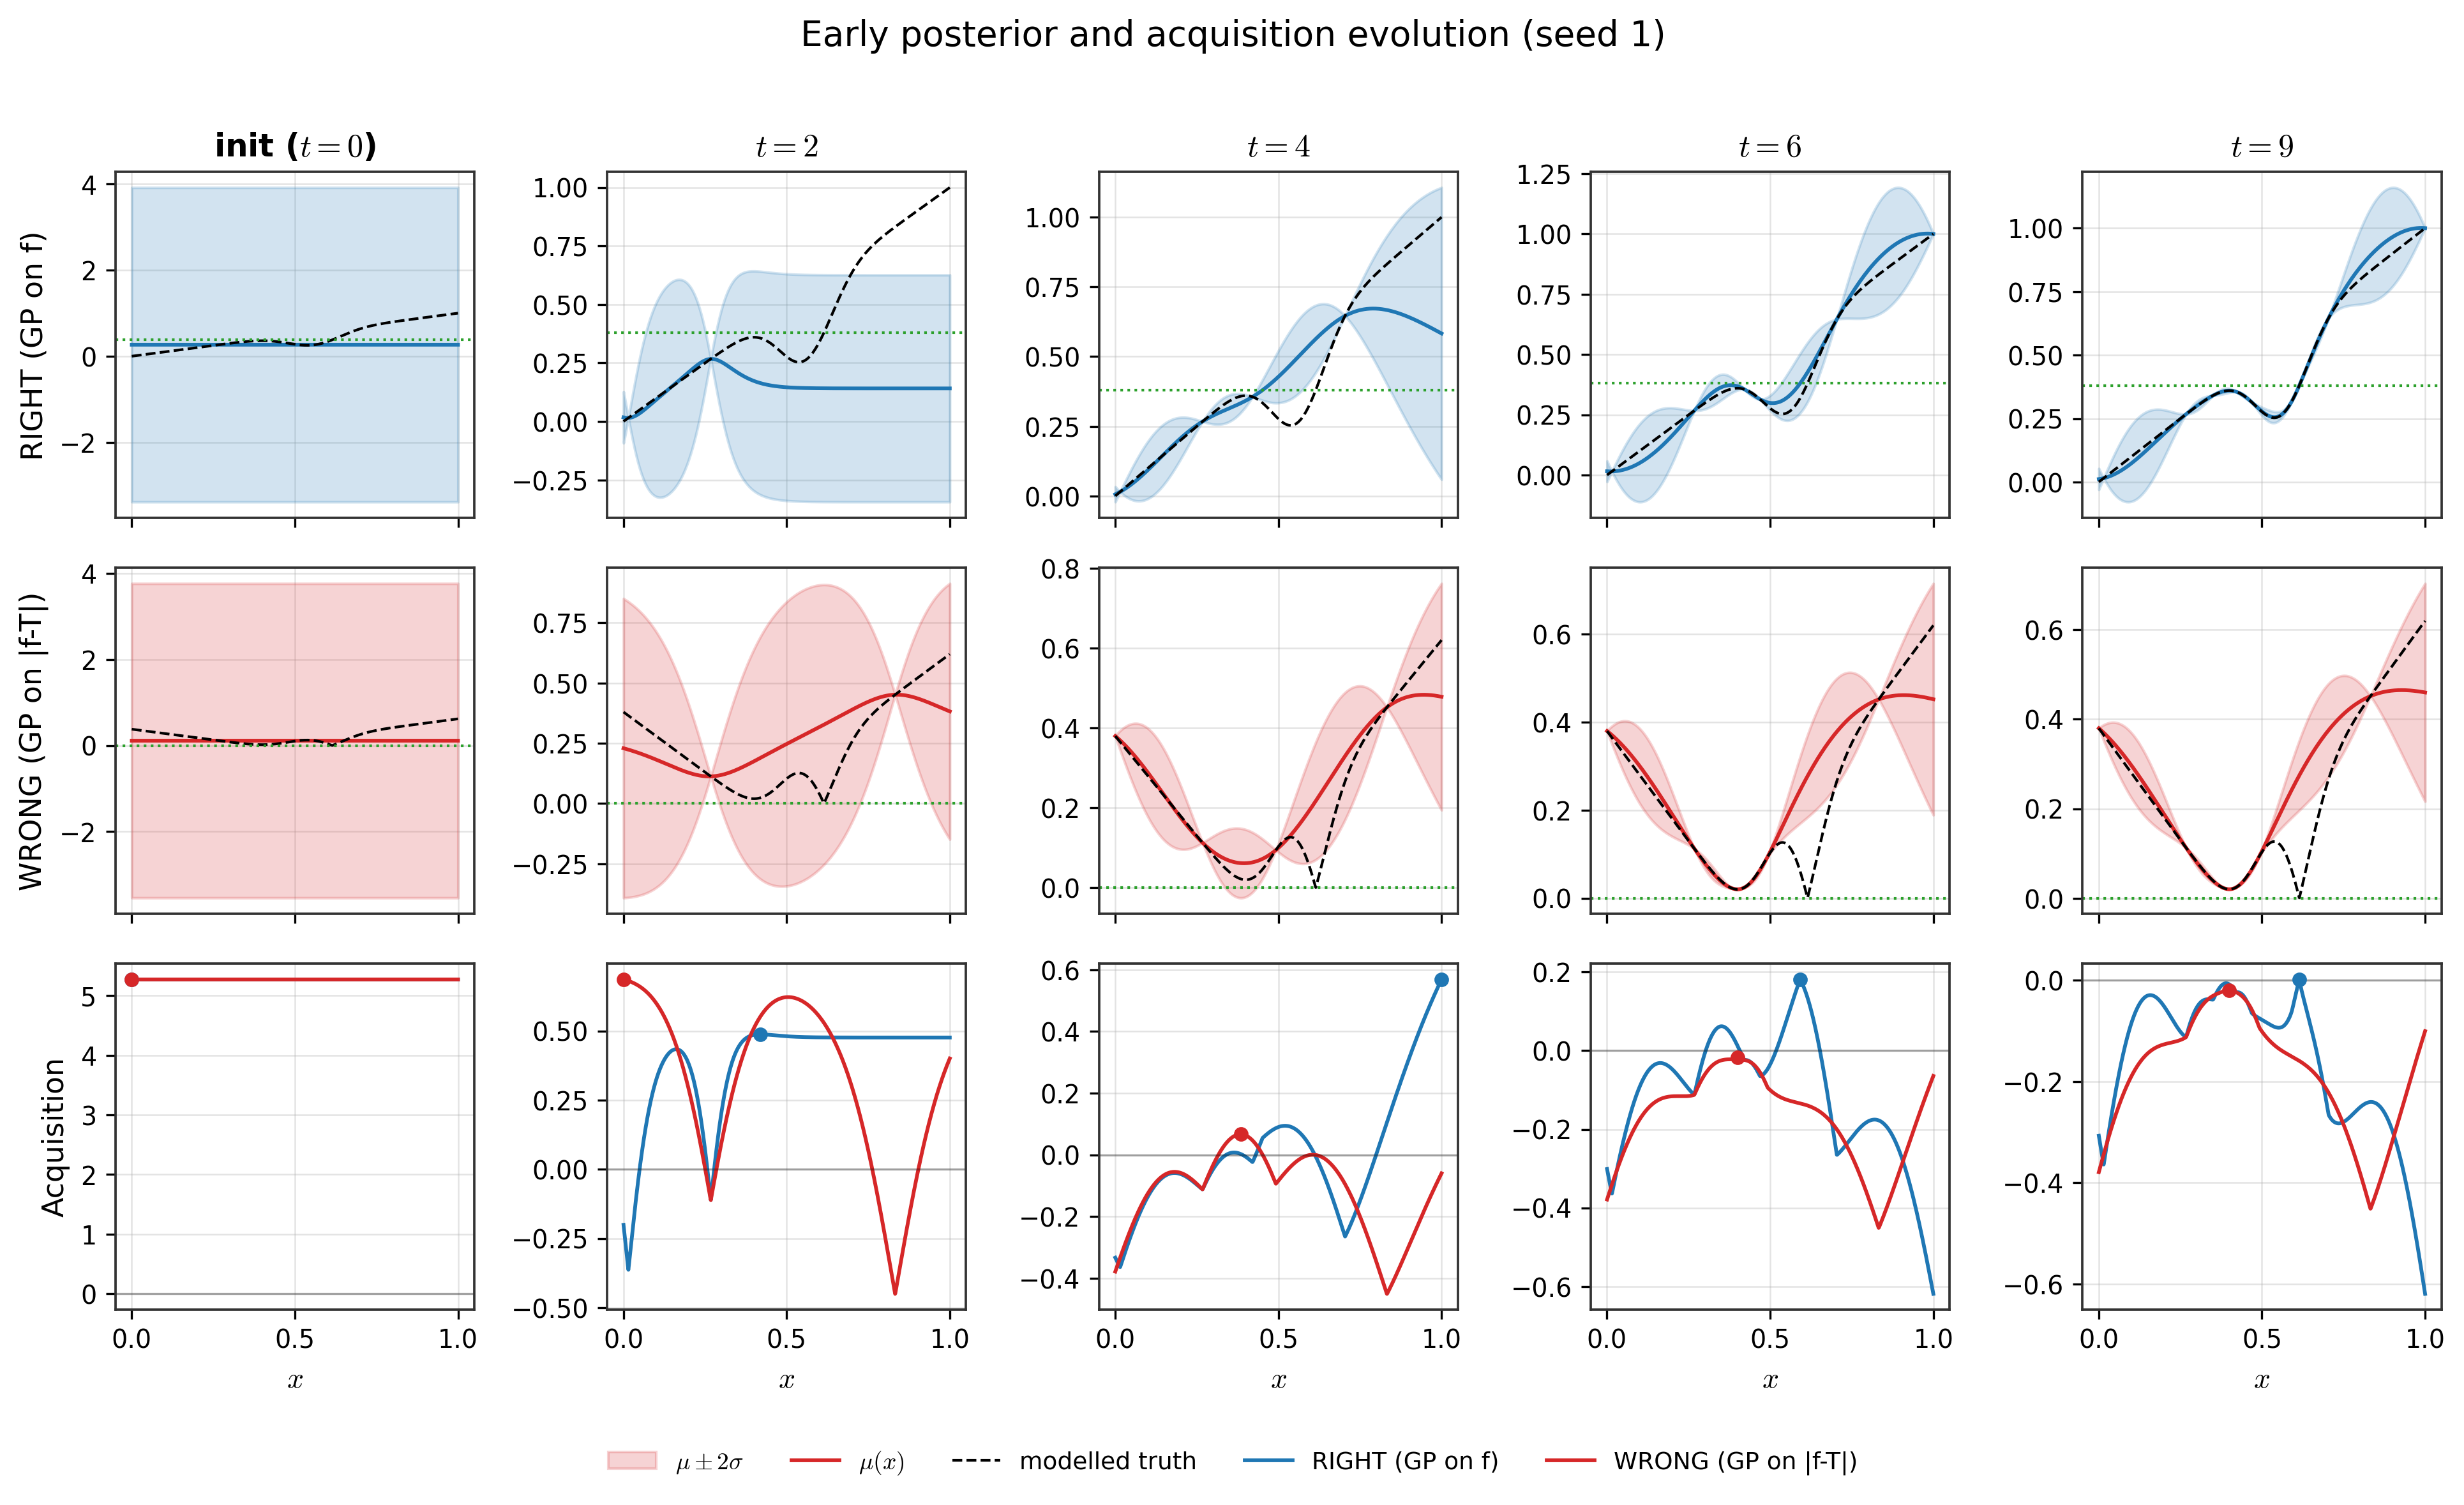
\includegraphics[width=1\linewidth]{figures/EXPA/02b_early_posterior_and_acquisition_evolution_gt.png}
    \caption{Trajectories on the Gaussian Trap 1d function. While RIGHT manages to reconstitute the landscape by $t=5$, WRONG's approximation of the function gets trapped in the gaussian well, and cannot find the actual optimum.}
    \label{fig:trajectories}
\end{figure}

\begin{figure}
    \centering
    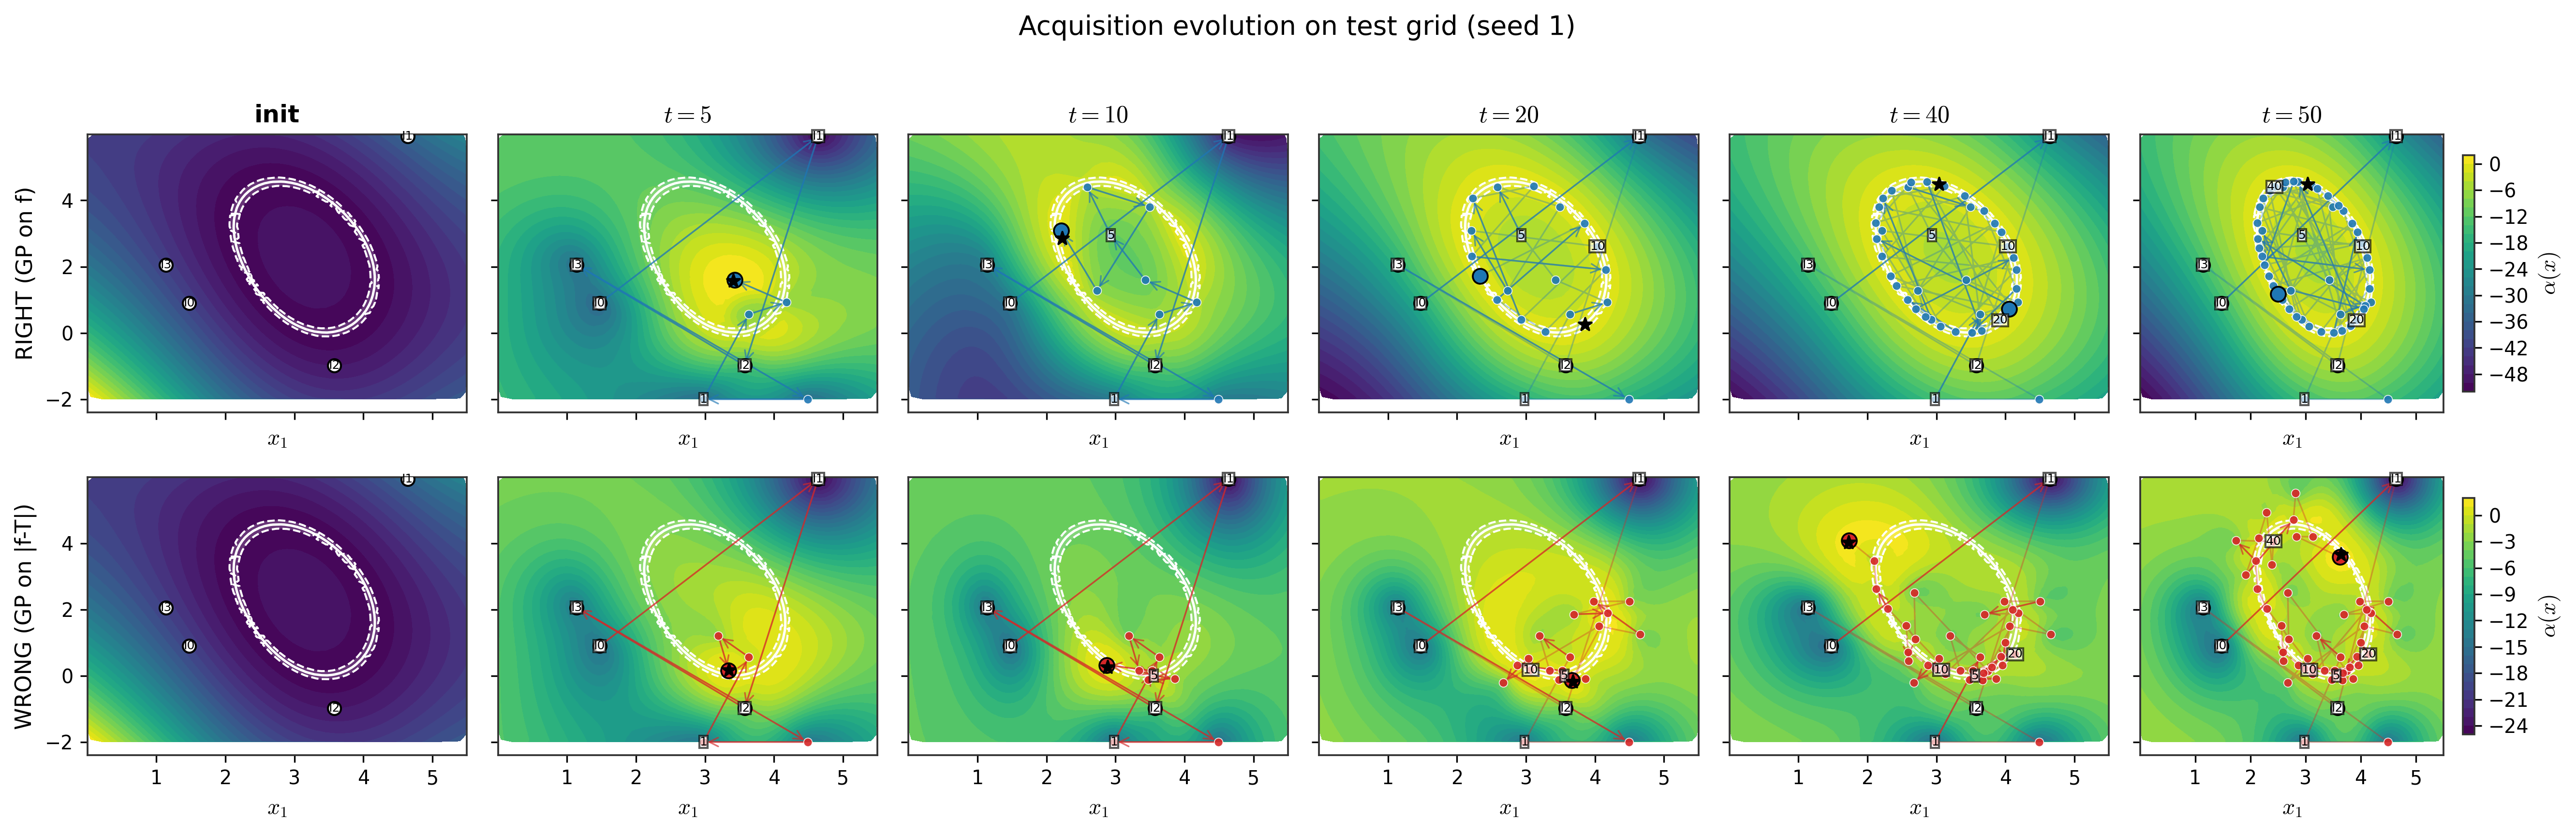
\includegraphics[width=1\linewidth]{figures/EXPA/02_acquisition_evolution_2d.png}
    \caption{Trajectories on the Branin 2d function. RIGHT reconstitutes the landscape very well while wrong queries remain uncertain until t=50, causing regret.}
    \label{fig:placeholder}
\end{figure}

\begin{figure}[htbp]
  \centering
  \begin{subfigure}[b]{0.32\linewidth}
    \centering
    \figph[\linewidth]{figures/EXPA/03_cumulative_regret_gaussian_trap.png}
    \caption{Cumulative regret, Gaussian trap.}
  \end{subfigure}\hfill
  \begin{subfigure}[b]{0.32\linewidth}
    \centering
    \figph[\linewidth]{figures/EXPA/03_failure_rate_gaussian_trap.png}
    \caption{Failure rate ($0.05$ vs $0.87$).}
  \end{subfigure}\hfill
  \begin{subfigure}[b]{0.32\linewidth}
    \centering
    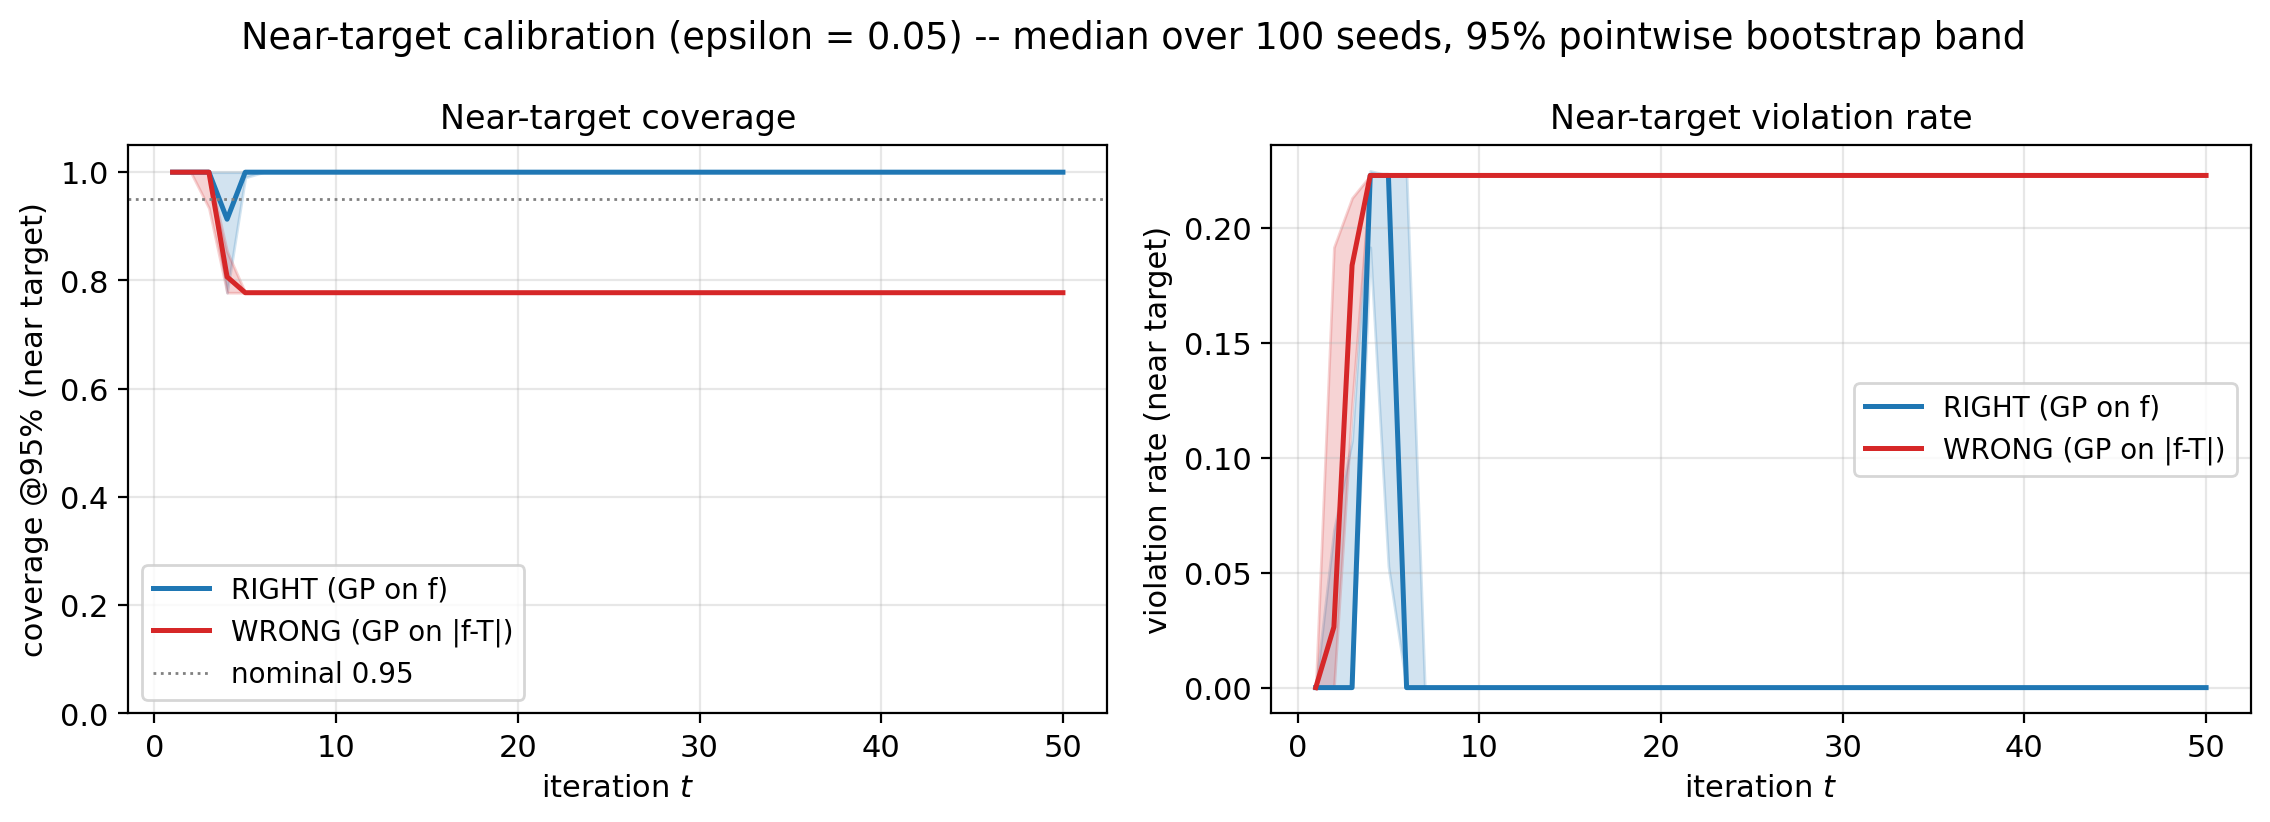
\includegraphics[
      width=\linewidth,
      keepaspectratio
    ]{figures/EXPA/04_near_target_calibration.png}
    \caption{Near target calibration interval violation.}
  \end{subfigure}

  \caption{\textbf{Aggregated results, Experiment~A} ($100$ seeds, median with
  $95\%$ bootstrap bands). The gap in regret is sharpest on the deceptive 1-D trap. Colours: blue $=$ \RIGHT{} (GP on $f$), red $=$ \WRONG{}
  (GP on $\abs{f-T}$).}
  \label{fig:tm-trap}
\end{figure}

\begin{figure}[htbp]
  \centering
  \begin{subfigure}[b]{0.32\linewidth}
    \centering
    \figph[\linewidth]{figures/EXPA/03_cumulative_regret_branin.png}
    \caption{Cumulative regret, Branin 2d.}
  \end{subfigure}\hfill
  \begin{subfigure}[b]{0.32\linewidth}
    \centering
    \figph[\linewidth]{figures/EXPA/03_final_distribution_branin.png}
    \caption{Final regret distribution Branin 2d.}
  \end{subfigure}\hfill
  \begin{subfigure}[b]{0.32\linewidth}
    \centering
    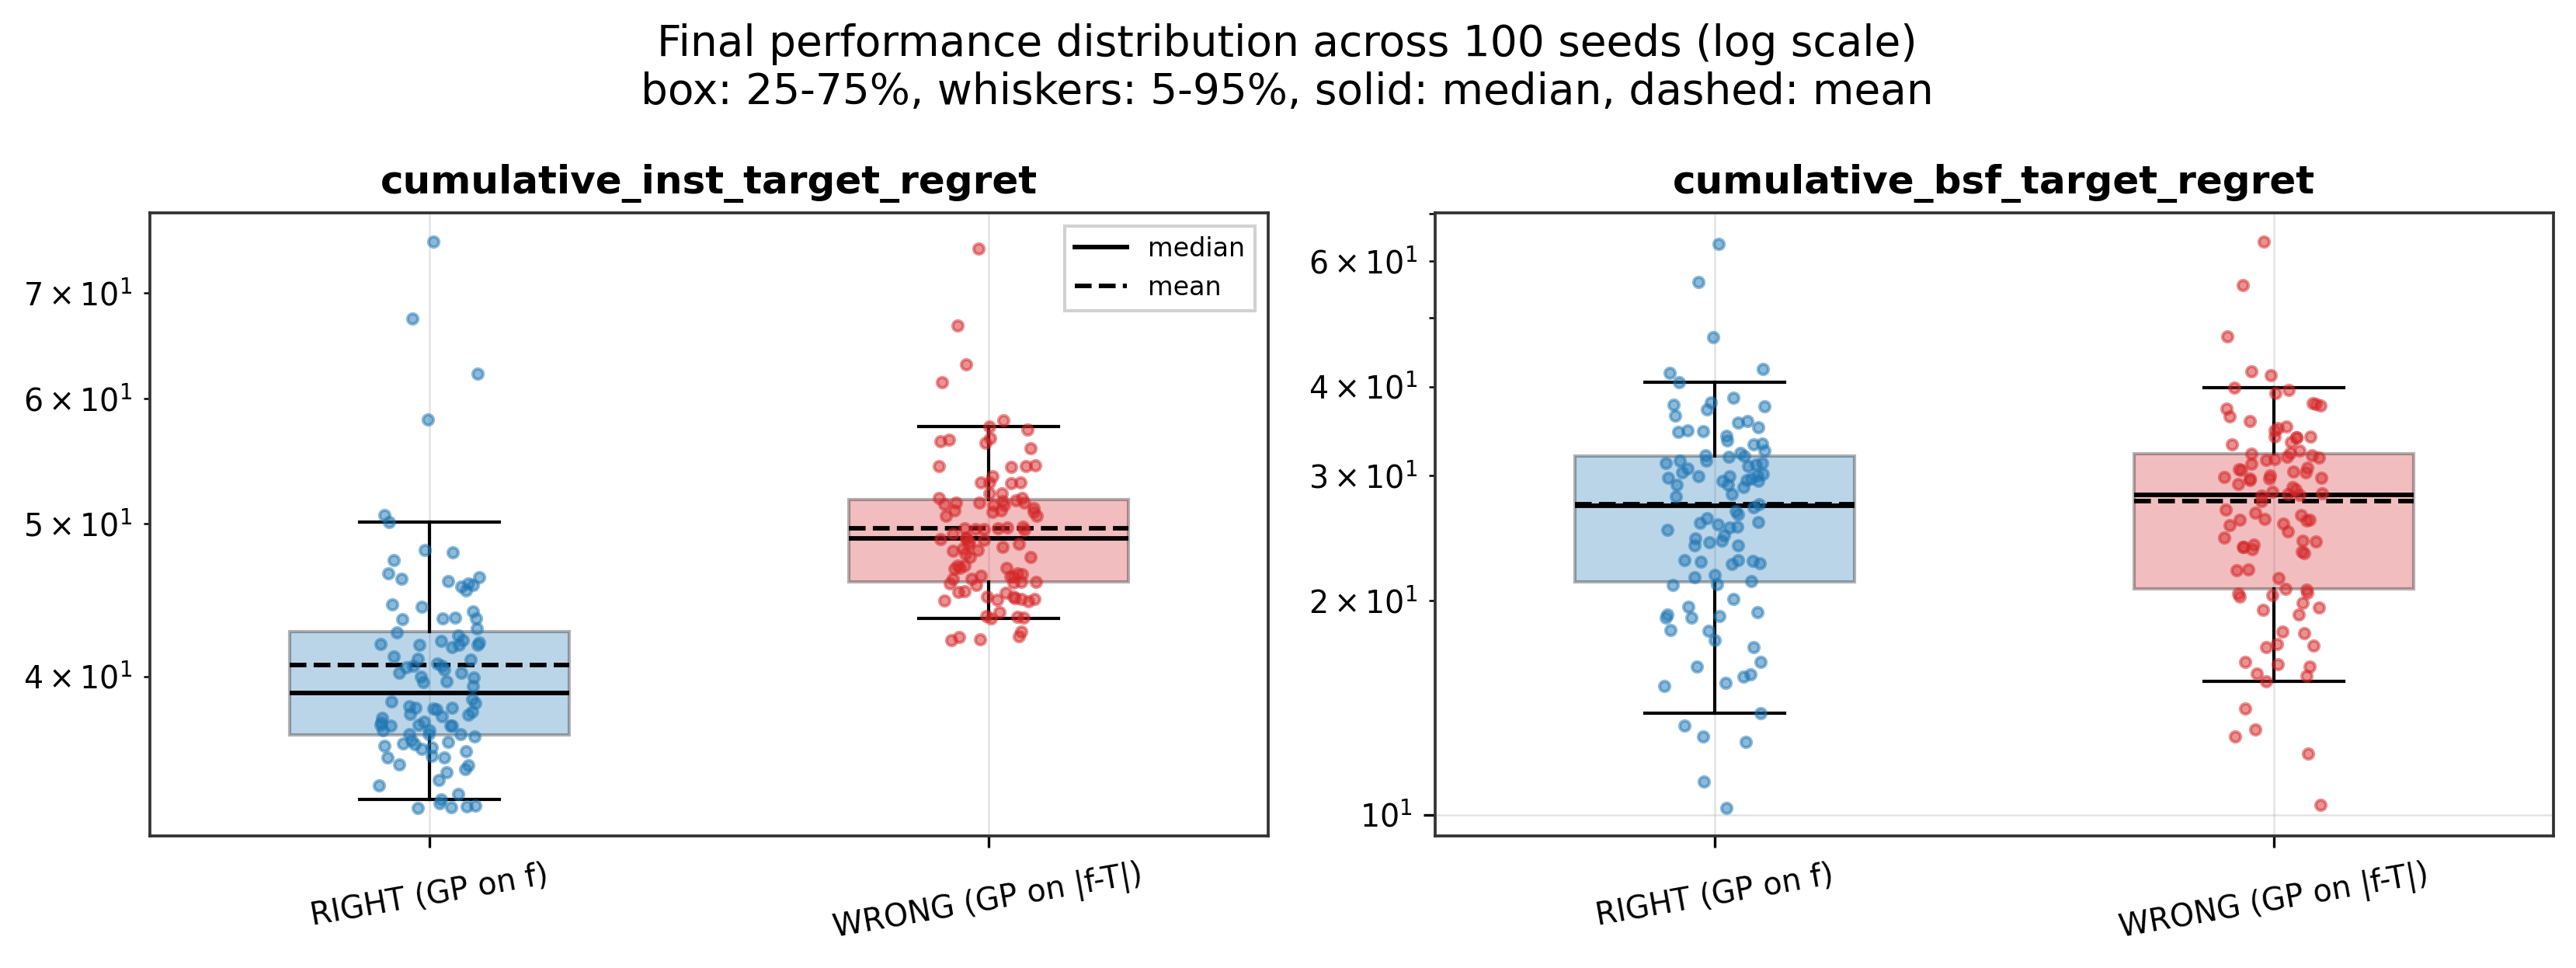
\includegraphics[
      width=\linewidth,
      keepaspectratio
    ]{figures/EXPA/03_final_distribution_hartmann.png}
    \caption{Final regret distribution Hartmann 6d}
  \end{subfigure}

  \caption{\textbf{Aggregated results, Experiment~A} ($100$ seeds, median with
  $95\%$ bootstrap bands). The gap in regret narrows with dimension. Colours: blue $=$ \RIGHT{} (GP on $f$), red $=$ \WRONG{}
  (GP on $\abs{f-T}$).}
  \label{fig:tm-dims}
\end{figure}